\section{Identification of wave spectrum model}

In this part we will analyze the model for the wave spectrum used as a disturbance in our simulations of the system. We will first extract the disturbance data and use it to empirically estimate a Power Spectral Density function for the model, then compare it to the theoretically obtained PSD-function. We will denote the empirically found PSD-function with $S(\omega)$ and the analytically derived one with $P(\omega)$.

\subsection{Problem a}

When estimating the Power Spectral Density function of $\psi_w$, $S_{\psi_w}(\omega)$, we load the "wave.mat" file containing the signals used for the wave disturbance. We used the MATLAB function \texttt{[Sxx, f] = pwelch(x, window, noverlap, nfft, fs)} and converted the result to the correct units, as shown in the MATLAB code in \cref{fig:p5p2} in \cref{sec:MATLAB}.
 
This gave us two vectors of data, Sxx and f, and plotting them against one another (plotting $S_{xx}(f)$)  with \texttt{plot(f, Sxx)} gives us what we are looking for. The result can be seen in \cref{fig:p5p2_PSD} marked as the empirically found function.
We can then analyze the plot and extract the information we need to look at the corresponding theoretical representation.


\subsection{Problem b}


We now want to derive the theoretical PSD-function of the wave spectrum.

We state \cref{eq:ship_model_xi} in the ship model as \cref{eq:xi}, 

\begin{equation} \label{eq:xi}
    \frac{d}{dt} \xi_w = \psi_w
    \quad \implies \quad \xi_w = \int \psi_w dt
\end{equation}

and combining it with \cref{eq:ship_model_psi_w} we get an equation for $\dot{\psi_w}$ given by \cref{eq:psi_dot}

\begin{equation} \label{eq:psi_dot}
    \dot{\psi_w} = - \omega_0  \int \psi_w dt - 2 \lambda \omega_0 \psi_w + K_w w_w
\end{equation}

Laplace transforming and reorganizing \cref{eq:psi_dot} gives us the transfer function from $w_w$ to $\psi_w$ in \cref{eq:H_w}

\begin{equation} \label{eq:H_w}
    \frac{\psi_w(s)}{w_w(s)} = H_w(s) = \frac{s K_w}{s^2 + s 2 \lambda \omega_0 + \omega_0^2}
\end{equation}


Then from the theoretical relation in \cref{eq:PSD_input_output_theory}, which in our case is stated in \cref{eq:PSD_input_output}, we arrive at \cref{eq:P_psi} because $w_w$ is white noise so $P_{w_w}(\omega) = 1$. 

\begin{equation} \label{eq:PSD_input_output_theory}
    S_y(\omega) = |H(j \omega)|^2 S_u(\omega), 
    \quad \textrm{where} \quad
    H(j \omega) = \frac{y(j \omega)}{u(j \omega)}
\end{equation}



\begin{equation} \label{eq:PSD_input_output}
    P_{\psi_w}(\omega) = |H_w(j \omega)|^2 P_{w_w}(\omega)
\end{equation}



\begin{equation} \label{eq:P_psi}
    P_{\psi_w}(\omega) = |H_w(j \omega)|^2 = \underline{\frac{\omega^2 K_w^2}{(\omega^2-\omega_0^2)^2 +(2\lambda \omega \omega_0)^2}}
\end{equation}

\subsection{Problem c}

Analyzing the power spectral density function obtained through MATLAB we get the values in \cref{eq:PSD_defining_values}.

\begin{equation} \label{eq:PSD_defining_values}
    \omega_0 = 0.4915 %\textrm{ rad/s}
    , \quad \sigma^2 = S_{\psi_w}(\omega)_{peak} = 0.0015 
    %\textrm{ J/rad}
\end{equation}

This means that the wave spectrum's influence is greatest when the waves have a frequency of $\omega_0$.



\begin{figure}
	\centering
	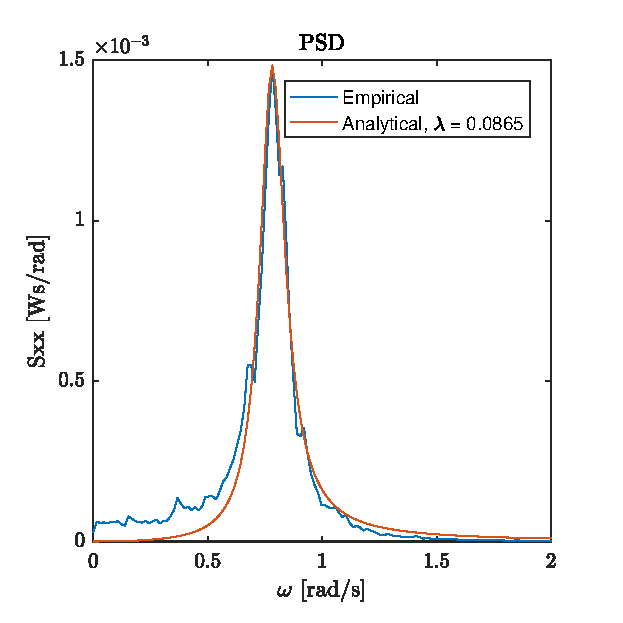
\includegraphics{figures/Ass2_PSD.eps}
	\caption{PSD function}
\label{fig:p5p2_PSD}
\end{figure}

\subsection{Problem d}
Now that we have two representations of the PSD-function for the wave spectrum, we want to match them together as best we can.

Given that $K_w = 2 \lambda \omega_0 \sigma$ we put it into \cref{eq:P_psi} and get \cref{eq:P_psi_Kw}

\begin{equation} \label{eq:P_psi_Kw}
    P_{\psi_w}(\omega, \lambda) = \underline{\frac{(2 \lambda \omega \omega_0 \sigma)^2}{(\omega^2-\omega_0^2)^2 +(2\lambda \omega \omega_0)^2}}
\end{equation}

We then use the MATLAB function \texttt{lsqcurvefit(Pxx, 0.1, f, Sxx)} to estimate $\lambda$ by minimizing the error between the emprically estimated $S_{\psi_w}(\omega)$ and the analytically derived $P_{\psi_w}(\omega, \lambda)$.

The result of the estimation was $\lambda = 0.0865$ and the comparison can be seen in \cref{fig:p5p2_PSD}.

\subsection{Evaluation of results}

In this section we are extracting and analyzing all the data available to us regarding the wave spectrum, and we are using a curve-fitting method which surpasses anything we can do ourselves. There is not much we can find to be improved upon in the methodology here.